\documentclass[10pt, a5paper]{article}
\usepackage{pdfpages}
\usepackage{parallel}
\usepackage[T2A]{fontenc}
\usepackage{ucs}
\usepackage[utf8x]{inputenc}
\usepackage[polish,english,russian]{babel}
\usepackage{hyperref}
\usepackage{rotating}
\usepackage[inner=2cm,top=1.8cm,outer=2cm,bottom=2.3cm,nohead]{geometry}
\usepackage{listings}
\usepackage{graphicx}
\usepackage{wrapfig}
\usepackage{longtable}
\usepackage{indentfirst}
\usepackage{array}
\newcolumntype{P}[1]{>{\raggedright\arraybackslash}p{#1}}
\frenchspacing
\usepackage{fixltx2e} %text sub- and superscripts
\usepackage{icomma} % коскі ў матэматычным рэжыме
\PreloadUnicodePage{4}

\newcommand{\longpage}{\enlargethispage{\baselineskip}}
\newcommand{\shortpage}{\enlargethispage{-\baselineskip}}

\def\switchlang#1{\expandafter\csname switchlang#1\endcsname}
\def\switchlangbe{
\let\saverefname=\refname%
\def\refname{Літаратура}%
\def\figurename{Іл.}%
}
\def\switchlangen{
\let\saverefname=\refname%
\def\refname{References}%
\def\figurename{Fig.}%
}
\def\switchlangru{
\let\saverefname=\refname%
\let\savefigurename=\figurename%
\def\refname{Литература}%
\def\figurename{Рис.}%
}

\hyphenation{admi-ni-stra-tive}
\hyphenation{ex-pe-ri-ence}
\hyphenation{fle-xi-bi-li-ty}
\hyphenation{Py-thon}
\hyphenation{ma-the-ma-ti-cal}
\hyphenation{re-ported}
\hyphenation{imp-le-menta-tions}
\hyphenation{pro-vides}
\hyphenation{en-gi-neering}
\hyphenation{com-pa-ti-bi-li-ty}
\hyphenation{im-pos-sible}
\hyphenation{desk-top}
\hyphenation{elec-tro-nic}
\hyphenation{com-pa-ny}
\hyphenation{de-ve-lop-ment}
\hyphenation{de-ve-loping}
\hyphenation{de-ve-lop}
\hyphenation{da-ta-ba-se}
\hyphenation{plat-forms}
\hyphenation{or-ga-ni-za-tion}
\hyphenation{pro-gramming}
\hyphenation{in-stru-ments}
\hyphenation{Li-nux}
\hyphenation{sour-ce}
\hyphenation{en-vi-ron-ment}
\hyphenation{Te-le-pathy}
\hyphenation{Li-nux-ov-ka}
\hyphenation{Open-BSD}
\hyphenation{Free-BSD}
\hyphenation{men-ti-on-ed}
\hyphenation{app-li-ca-tion}

\def\progref!#1!{\texttt{#1}}
\renewcommand{\arraystretch}{2} %Іначай формулы ў матрыцы зліпаюцца з лініямі
\usepackage{array}

\def\interview #1 (#2), #3, #4, #5\par{

\section[#1, #3, #4]{#1 -- #3, #4}
\def\qname{LVEE}
\def\aname{#1}
\def\q ##1\par{{\noindent \bf \qname: ##1 }\par}
\def\a{{\noindent \bf \aname: } \def\qname{L}\def\aname{#2}}
}

\def\interview* #1 (#2), #3, #4, #5\par{

\section*{#1\\{\small\rm #3, #4. #5}}

\def\qname{LVEE}
\def\aname{#1}
\def\q ##1\par{{\noindent \bf \qname: ##1 }\par}
\def\a{{\noindent \bf \aname: } \def\qname{L}\def\aname{#2}}
}

\begin{document}
\title{Опыты над людьми и Octave: FOSS-based GSR measurements}
\author{Ольга Карабутова, Minsk, Belarus}
\maketitle
\begin{abstract}
The paper describes practical experience of creating a biometrical device to evaluate user’s stress level. Signs specific to stress are considered as well as the device prototype and intermediate research results. Free/libre open-source software used to evaluate and analyse raw biometric data is covered.
\end{abstract}
\subsection*{Вступление}

С каждым днем различные устройства, использующие биометрические данные (фитнес-гаджеты, сканеры отпечатков пальцев, умные часы, умные очки, одежда, протезы, управляемые силой мысли, нейрокомпьютерные интерфейсы) находят все более широкое применение, а сами устройства становятся меньше и удобнее для повседневного использования.

Перед нами стояла задача  создания биометрического устройства, которое могло бы отслеживать уровень стресса  человека в течение дня, недели.  Хотя обычно человек сам в состоянии определить, находится сейчас он в стрессовом состоянии или нет, но он далеко не всегда способен объективно оценить стрессовую  нагрузку на свой организм, тем более, не всегда очевидны причины стресса.

\subsection*{Стресс}

Под стрессом (от англ. stress "--- нажим, напряжение) понимают общую реакцию организма на физическое или психологическое воздействие, выводящее его из состояния равновесия (нарушающее гомеостаз), а также соответствующее состояние нервной системы и организма в целом.
«Изобретатель» стресса канадский эндокринолог Ганс Салье доказал, что стресс ведет к истощению организма и к очень многим нарушениям здоровья.

Реакцию организма на стресс можно выразить фразой «дерись или беги». За большинство физиологических изменений, отвечают две нейроэндокринные системы, управляемых гипоталамусом: симпатической и парасимпатической. Симпатическая нервная система подготавливает организм к атаке, обеспечивая выброс в кровь глюкозы, увеличение кислорода в крови и артериального давления, сердцебиения, расширяет зрачок, активирует железы и мускулатуру, сокращает ток периферических сосудов, а также подавляет деятельность большинства внутренних органов, такие как пищеварение. Действие парасимпатической системы во многом противоположно. Поэтому можно выделить стандартные признаки, сопутствующие стрессовой ситуации:

\begin{itemize}
  \item артериальное давление
  \item содержание сахара и кислорода в крови
  \item повышение частоты сердцебиения, учащение дыхания
  \item расширение зрачков
  \item специфическое сокращение лицевых нервов (мимика)
  \item уменьшение слюноотделения
\end{itemize}

С точки зрения использования в конечном устройстве для выявления стресса нас интересуют в первую очередь метрики, пригодные для неинвазивного измерения и обладающие при этом достаточной достоверностью.

Кожно-Гальваническая Реакция
Ряд исследований показывает, что для детектирования стресса достаточно одного датчика кожно-гальванической реакции (Galvanic Skin Response или GSR).

GSR "--- биоэлектрическая реакция, обусловленная деятельностью потовых желез. Если приложить к коже электрическое напряжение, то между двумя участками кожи можно замерить электрическое сопротивление или проводимость. Во время стрессового воздействия потовые железы кожи выделяют микрочастицы пота, в результате чего сопротивление кожи меняется. На рисунке показана идеальная реакция на стрессовый стимул, обозначенный красной линией с подписью «Stimulus». Можно заметить временную задержку отклика (Latency) и последующее время восстановления (Recovery), т.е. адаптации к новому гомеостазу или релаксации после точечного стресса.

\begin{figure}[h!]
  \centering
  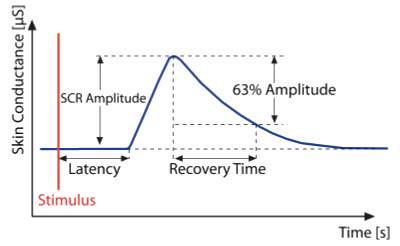
\includegraphics[width=\textwidth]{107_2014_w_Karabutova_plot.png}
\end{figure}

\subsection*{Устройство}

Разработка включает две части: носимое устройство в виде браслета и программное обеспечение, устанавливаемое на персональный компьютер или мобильное устройство.

Носимое устройство включает следующие части:

\begin{itemize}
  \item датчик GSR
  \item акселерометр
  \item микропроцессор
  \item память
  \item RF-модуль (Bluetooth Low Energy)
  \item устройство питания (батарея CR2032 или литий-полимерный аккумулятор)
\end{itemize}

Биометрия считывается с аналоговых датчиков, усиливается, конвертируется в цифровой сигнал. Далее показания агрегируются в памяти, находящейся на устройстве. При портативном ношении данные собираются на устройстве за продолжительный период времени. Также они могут передаваться в режиме реального времени на персональный компьютер или мобильное устройство для обработки "--- как по интерфейсу USB, так и через беспроводной интерфейс Bluetooth Low Energy, который широко используется в медицинских устройствах.

Для обработки данных на PC использован GNU Octave.

\begin{figure}[h!]
  \centering
  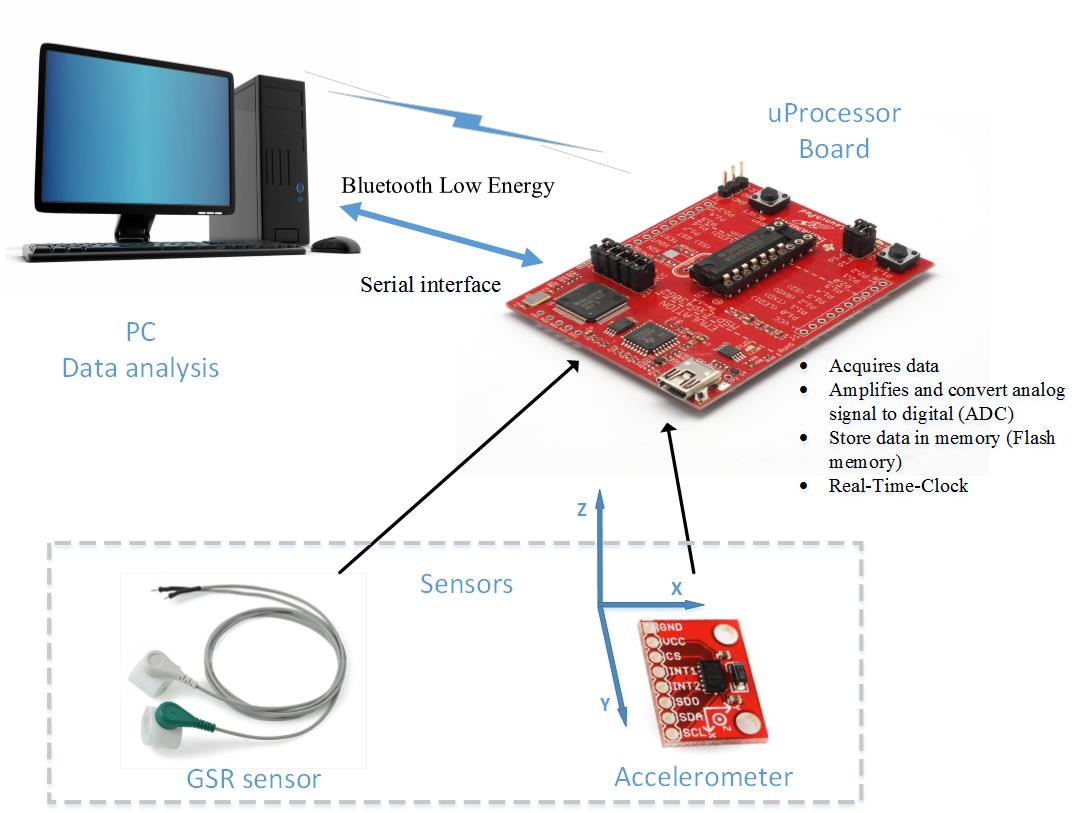
\includegraphics[width=\textwidth]{107_2014_w_Karabutova_struct.png}
\end{figure}

\subsection*{Методика тестирования}

Для проверки работоспособности прибора использовалась серия тестов следующего вида. После закрепления датчиков подопытному давался адаптационный период не менее 15 минут. Далее испытуемый подвергается стрессовым воздействиям, которые следовали одно за другим в случайном порядке. Воздействия проводились с перерывом в 20—30 минут. Между последним стрессовым воздействием и завершением предусматривалась пауза не менее 10—15 минут. Общая продолжительность одной сессии составляет 1—3 часа.

Датчики GSR крепятся на двух пальцах одной руки или на запястье подопытного, но должны быть разнесены минимум на 1 сантиметр расстояния между ними, с обеспечением плотного контакта. Плотность контакта на пальцах обеспечивается заводским креплением на «липучке», а на запястье "--- креплением на резинке с регулируемой длиной браслета. Дополнительно на теле человека закрепляется акселерометр.

В качестве типов стрессовой нагрузки применялись следующие:

\begin{table}[t!]
  \centering
  \begin{tabular}{P{10em}|P{20em}}
    \hline
    Физическое воздействие & Физические упражнения \\
     & Изменение температуры в помещении \\
    \hline
    Когнитивная нагрузка & Решение интересных, но не тривиальных задач \\
     & Прохождение/выполнение задач вне компетенции на время \\
     & Соревновательные игры \\
    \hline
    Эмоциональная нагрузка & Видеоролики или материалы, вызывающие эмоциональный отклик \\
     & Обсуждение событий, вызывающих радость, положительные эмоции \\
     & Требование отчета вышестоящим начальником (этот тест показал слабую эффективность) \\
     & Ситуация экзамена \\
    \hline
  \end{tabular}
\end{table}
Данные с датчиков сохранялись в cvs-файл и затем обрабатывались в Octave. Там же обработанные данные пропускались через алгоритм, выдающий на выходе, когда у человека был стресс (по показаниям GSR), и был ли он вызван физической активностью или нет (по показаниям акселерометра).

\begin{figure}[h!]
  \centering
  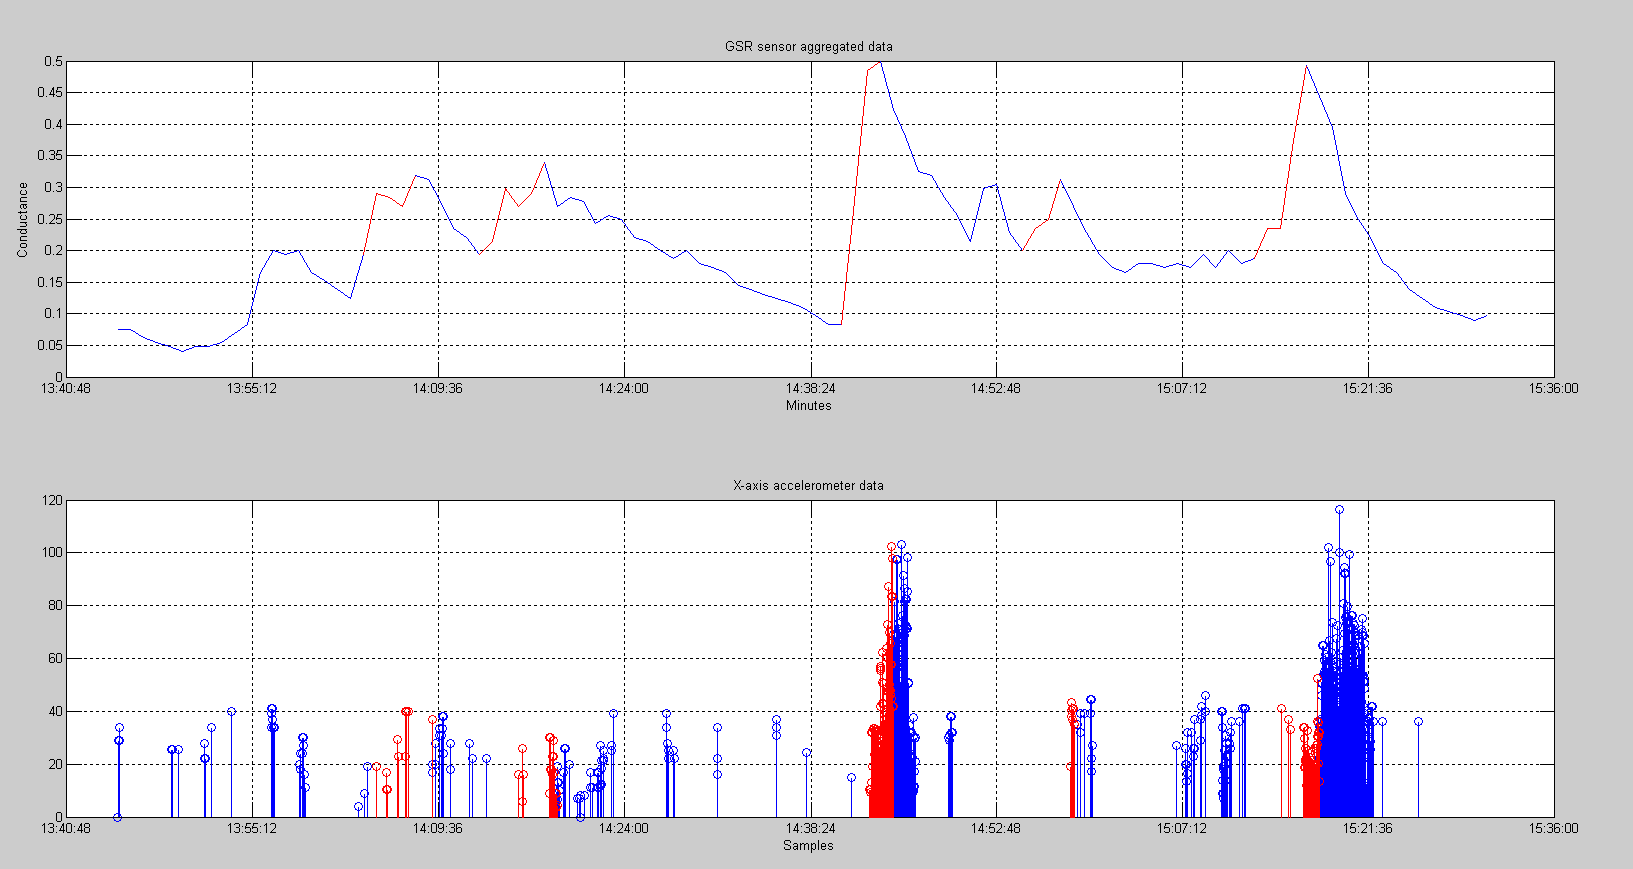
\includegraphics[width=\textwidth]{107_2014_w_Karabutova_data.png}
\end{figure}

Параллельно все происходящее во время опытов тщательно документировалось наблюдателем. Пример журнала:

\begin{verbatim}
13.57	Испытуемый разговаривает по телефону 
Виден пик повышения GSR, но как стресс программа это не выделила (не достаточно существенное отклонение от общего уровня GSR)
14.05	Игра «Морской бой» с ограничением по времени
14.09 	Окончание игры
14.10 	Обсуждение игры и тактик. (Испытуемый выиграл)
14.44	Физическое упражнение  «бег на месте»
Стресс, вызванный физической активностью испытуемого, легко отличить по показаниям акселерометра
14.45	Завершение физических упражнений
15.00	Включение обогревателя в комнате
15.16	Выполнение разнообразных физических упражнений
15.21	Завершение физических упражнений
\end{verbatim}

\subsection*{Результаты испытаний}

Тестирование показало, что стресс, вызванный физической нагрузкой, детектируется 100\%. Что касается прочих причин, было сложно иногда создать однозначно стрессовую ситуацию для подопытного.
Например, ситуация отчета перед начальством не всегда вызывала у подопытного волнение (подопытному было известно, что он в ситуации «теста» и ситуация создана искусственно).
Тем не менее, у разработчика, который также иногда выступал в роли подопытного, сообщение о визите вышестоящего начальства, как и сам визит, однозначно повышало регистрируемый уровень стресса.

Игровые ситуации дают однозначный результат, как и во время игры, так и при последующих обсуждениях результатов и стратегий. Аналогично дело обстоит и с просмотром видеоматериалов, вызывающих с высокой долей вероятности эмоциональный отклик у реципиентов.

\subsection*{Octave}

GNU Octave "--- свободная система для математических вычислений, использующая совместимый с MATLAB язык высокого уровня.
По сути, Octave "--- это свободный клон MATLAB, благодаря чему и динамически подгружаемые модули (*.m-файлы), и пользовательские функции можно очень легко портировать из одной среды в другую.

В среде профессиональных исследователей MATLAB занимает лидирующие позиции (благодаря крайне обширному набору вычислительных функций практически для всех областей применения) а к его свободным клонам часто относятся с предубеждением. Однако по нашему опыту GNU Octave оказался чрезвычайно мощным математическим инструментом, с помощью которого можно экспериментировать, моделировать устройства и обрабатывать цифровые данные.

Не в последнюю очередь это достигается благодаря тому, что Octave позволяет подключать сторонние утилиты, а также общие или предметно-ориентированные библиотеки функций для вычислений. 
Например, для построения графиков по умолчанию Octave использует Gnuplot, хотя также есть на выбор не менее 5 альтернативных графических пакетов.

Сторонняя библиотека Octave-forge включает множество пакетов, среди которых для решения класса задач анализа биометрических данных нами были отобраны следующие:

\textbf{Для получения данных из подключаемых устройств:}

\begin{itemize}
  \item \textbf{instrument-control} позволяет взаимодействовать с внешними устройствами через последовательный и параллельный порты, I²C, TCP/IP, интерфейсы GPIB, VXI11 и USBTMC.
  \item \textbf{communications} "--- передача цифровых данных, кодов коррекции ошибок ECC, модуляции и поля Галуа.
\end{itemize}

\textbf{Для цифровой обработки сигнала:}

\begin{itemize}
  \item \textbf{signal} "--- наборы функций для обработки сигналов (а также обработки изображений, проектирования цифровых фильтров и систем связи -- БПФ, фильтры различных порядков).
  \item \textbf{ltfat} "--- библиотека частотно-временного анализа сигналов. Позволяет производить большое количество линейных преобразований, включая преобразование Габора и вейвлет-преобразование, а так же шаблоны для конструирования окон (моделирование фильтров) и утилиты для манипулирования коэффициентами.
\end{itemize}

\textbf{Для статистики, анализа данных и машиного обучения:}

\begin{itemize}
  \item \textbf{nan} "--- набор утилит для статистики и машинного обучения, работает как с Octave, так и с Matlab, умеет обрабатывать как непрерывные данные, так и данные с пропущенными значениями.
  \item \textbf{mvn} "--- кластеризация многомерного нормального распределения
  \item \textbf{fuzzy-logic-toolkit} позволят создавать экспертные системы на основе нечеткой логики, проводить кластеризацию нечеткими алгоритмами, а также проектировать нечеткие нейронные сети.
  \item \textbf{fl-core} содержит базовые функции для нечеткой логики.
  \item \textbf{queueing} содержит набор функций в том числе и для анализа цепей Маркова
\end{itemize}

В итоге для решения нашей задачи был задействован меньший набор пакетов Octave для построения эффективной обработки данных и ее статистического анализа (преимущественно использовались пакеты signal). Определенно мог быть задействован пакет instrument-control для приема данных на ПК.
Но Octave "--- поистине мощный математический инструмент, с помощью которого можно экспериментировать, моделировать устройства и обрабатывать цифровые данные.

\end{document}
